\documentclass{article}

% Language setting
% Replace `english' with e.g. `spanish' to change the document language
\usepackage[portuguese]{babel}

% Set page size and margins
% Replace `letterpaper' with `a4paper' for UK/EU standard size
\usepackage[letterpaper,top=2cm,bottom=2cm,left=3cm,right=3cm,marginparwidth=1.75cm]{geometry}

% Useful packages
\usepackage{amsmath}
\usepackage{graphicx}
\usepackage[colorlinks=true, allcolors=blue]{hyperref}

\title{Exercício Programa 04 - Aproximação de Modelo Estatístico Multinomial m-dimensional}
\author{Alexandre Barsam Junqueira - NºUSP: 12561642\\Guilherme Lloret Cavalcante - NºUSP: 14576152}

\begin{document}
\maketitle

\begin{abstract}
Esse relatório busca aplicar o método de Markov Chain Monte Carlo para obter uma aproximação de um Modelo Estatístico Multinomial m-dimensional por meio de uma interpolação polinomial $U(v)$ que aproxime a função verdade do modelo $W(v)$.

\end{abstract}

\section{Modelo Estatístico}
Considere o modelo estatístico multinomial $m$-dimensional com observações $x$, informação a priori $y$ e parâmetro $\theta$, $x,y \in \mathbb{N}^m$, $\theta \in \Theta = S^m = \{\theta \in \mathbb{R}^m_+ : \theta^T \mathbf{1} = 1\}$. Esse modelo estatístico é composto pelas seguintes igualdades.

Potencial a posteriori:
\[ f(\theta \mid x,y) = \prod_{i=1}^{m} \theta^{x_i + y_i - 1}_i \]

Conjunto de corte:
\[ T(v) = \{\theta \in \Theta : f(\theta \mid x,y) \leq v\}, \quad v \geq 0 \]

Função verdade:
\[ W(v) = \int_{T(v)} f(\theta \mid x,y) d\theta \]

$W(v)$ é a massa de probabilidade a posteriori dentro de $T(v)$, ou seja, a massa de probabilidade onde o potencial a posteriori, $f(\theta \mid x,y)$, não excede a cota $v$. O objetivo é obter uma função $U(v)$ que aproxime adequadamente a função $W(v)$ com $\epsilon \leq 0.05\%$.

\section{Abordagem do Problema}
A solução consiste nas seguintes etapas:

\begin{enumerate}
    \item Defina $k$ pontos de corte, $0=v_0 < v_1 < \cdots < v_k = \sup f(\theta)$, da seguinte forma:

    \item Use uma Cadeia de Markov com o núcleo baseado em uma distribuição normal multivariada $N(0,\Sigma)$, com a matriz de covariância baseada no parâmetro $a$ da distribuição de Dirichlet para gerar pontos na região $\Theta$. 
    
    \item Use a fração de pontos simulados $\theta_t$ dentro de cada bin, $v_{j-1} < f(\theta_t) < v_j$, como uma aproximação de $W(v_j) - W(v_{j-1})$.
    
    \item Ajuste dinamicamente as bordas de cada bin, $v_j$, para obter bins com pesos aproximadamente iguais, isto é, $W(v_j) - W(v_{j-1}) \approx \frac{1}{k}$.
    
    \item Obtenha como saída uma função $U(v)$ que dê uma boa aproximação de $W(v)$.
\end{enumerate}

\subsection{Gerando Pontos utilizando a Cadeia de Markov}
\subsubsection{Algorítmo de Metropolis-Hastings}
 O objetivo por trás deste algorítmo é gerar uma cadeia de amostras que converge para a distribuição que se deseja estimar. A cada iteração, o método propõe um novo ponto tendo como base, neste caso, a distribuição normal multivariada (com a matriz de covariância definida com base no parâmetro $a$ da Distribuição de Dirichlet). Além disso, o método é responsável por aceitar ou rejeitar cada um dos novos pontos gerados com base em uma taxa de aceitação, que é calculada da seguite forma:
\\
\[
\theta_{t+1} = \min\left(1, \frac{p(\theta_{t+1})q(\theta_{t}|\theta_{t+1})}{p(\theta_{t})q(\theta_{t+1}|\theta_{t})}\right)
\]

Onde:
\begin{itemize}
    \item \( p(\theta_{t}) \) é a distribuição de probabilidade alvo,
    \item \( q(\theta_{t+1}|\theta_{t}) \) é a distribuição de probabilidade da proposta,
    \item \( \theta_{t+1} \) é a nova amostra proposta no passo \( t+1 \),
    \item \( \theta_{t} \) é a amostra atual no passo \( t \).
\end{itemize}

Esse processo permite a geração um maior número de pontos nas regiões de alta probabilidade na distribuição-alvo.
 
\subsubsection{Ajuste do Núcleo $N(0, \Sigma)$}
Com o intuito de otimizar o núcleo do Markov Chain Monte Carlo, $\Sigma$ foi determinada por meio de $\alpha$, isto é, as observações $x$ e a informação \textit{a priori} $y$. Na diagonal principal ($M_{i, i}$), colocou-se $\sigma^{2}(\alpha_i)$. Já quando $M_{i, j}$, com $i \not= j$, utilizou-se $Cov(\alpha_i, \alpha_j)$.

Além disso, para garantir que as amostras geradas estavam no simplex $\Theta$, impôs-se algumas restrições. Primeiramente, que cada elemento $\theta_i \geq 0$, além de que $\sum_{i = 1}^{k} = 1$. Isso pode ser feito por meio da definição da última coordenada como $1 - \sum_{i = 1}^{k - 1}$.

\subsubsection{Definição do \textit{burn-in}}


Para que o método funcione de forma eficiente, é necessário que o núcleo do MCMC seja ajustado, isto é, que haja uma garantia de que a estimativa gerada não dependerá do valor do ponto \(\theta_{\text{inicial}}\). Considerando que uma das propriedades das Cadeias de Markov é a falta de memória, isto é, dada uma matriz de transição, a geração de \(\theta_{t+1}\) depende apenas de \(\theta_{t}\), basta garantir que o \(\theta\) gerado esteja em uma região em que o potencial da distribuição seja considerado alto. Por essa razão, foi implementada a função \textbf{calcular\_burn\_in}.

Esta função tem por objetivo testar o potencial de cada um dos pontos da cadeia e calcular o seu respectivo potencial. Com base nisso, a função registra o maior potencial calculado e seleciona na cadeia o índice do primeiro ponto com um potencial de pelo menos 50\% do maior potencial observado. Caso não haja nenhum \(\theta_i\) que satisfaça tal condição, a função retornará o índice de maior potencial no primeiro quarto da lista.

Dessa forma, pode-se eliminar os pontos até tal índice e começar a cadeia pelo \(\theta_i\) selecionado por essa função, o que garante que o algoritmo inicie por um ponto com alto potencial.


\subsubsection{Definição do progresso do MCMC}
Com o intuito de definir a evolução e a qualidade do algoritmo MCMC utilizado, três abordagens principais foram utilizadas: diagnóstico de Gelman-Rubin ($\hat{R}$), \textit{trace plots}, auto-correlação e \textit{posterior plots}.

Análise de cada um dos indicadores:
\begin{enumerate}
    \item \textbf{Diagnóstico de Gelman-Rubin ($\hat{R}$:} compara a variação intra-cadeia com a variação inter-cadeias. Se as cadeias convergiram, esses valores devem ser semelhantes. Isso ocorre quando $\hat{R} \approx 1$.
    \item \textbf{Trace Plots:} são os gráficos dos valores amostrados ao longo das iterações. Um trace plot estável e "misturado" indica boa convergência.
    \item \textbf{Auto-Correlação:} mede a correlação entre os valores de uma cadeia em diferentes atrasos. Baixa autocorrelação (rápida queda para zero) indica boa mistura.
    \item \textbf{Posterior Plots:} mostra a distribuição dos valores de cada entrada do vetor $\theta$. Verificar se as distribuições parecem razoáveis e têm a forma esperada.
\end{enumerate}

Exemplo: para $\alpha = [3, 8, 13]$, obteve-se $\hat{R} = [1.001, 1.002, 1.001]$, com $n = 10^4$. Além disso, observando-se os gráficos.

\begin{figure}[h]
    \centering
    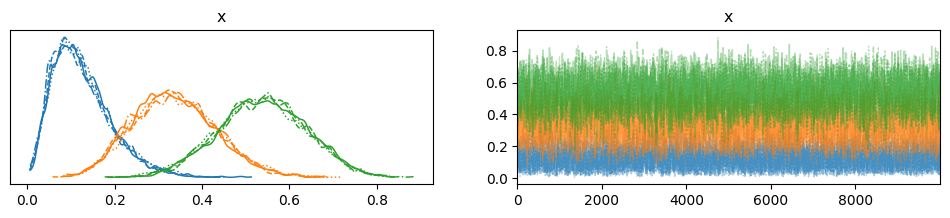
\includegraphics[width=0.5\linewidth]{Trace Plot.png}
    \caption{Trace Plots}
    \label{fig:enter-label}
\end{figure}

\begin{figure}[h]
    \centering
    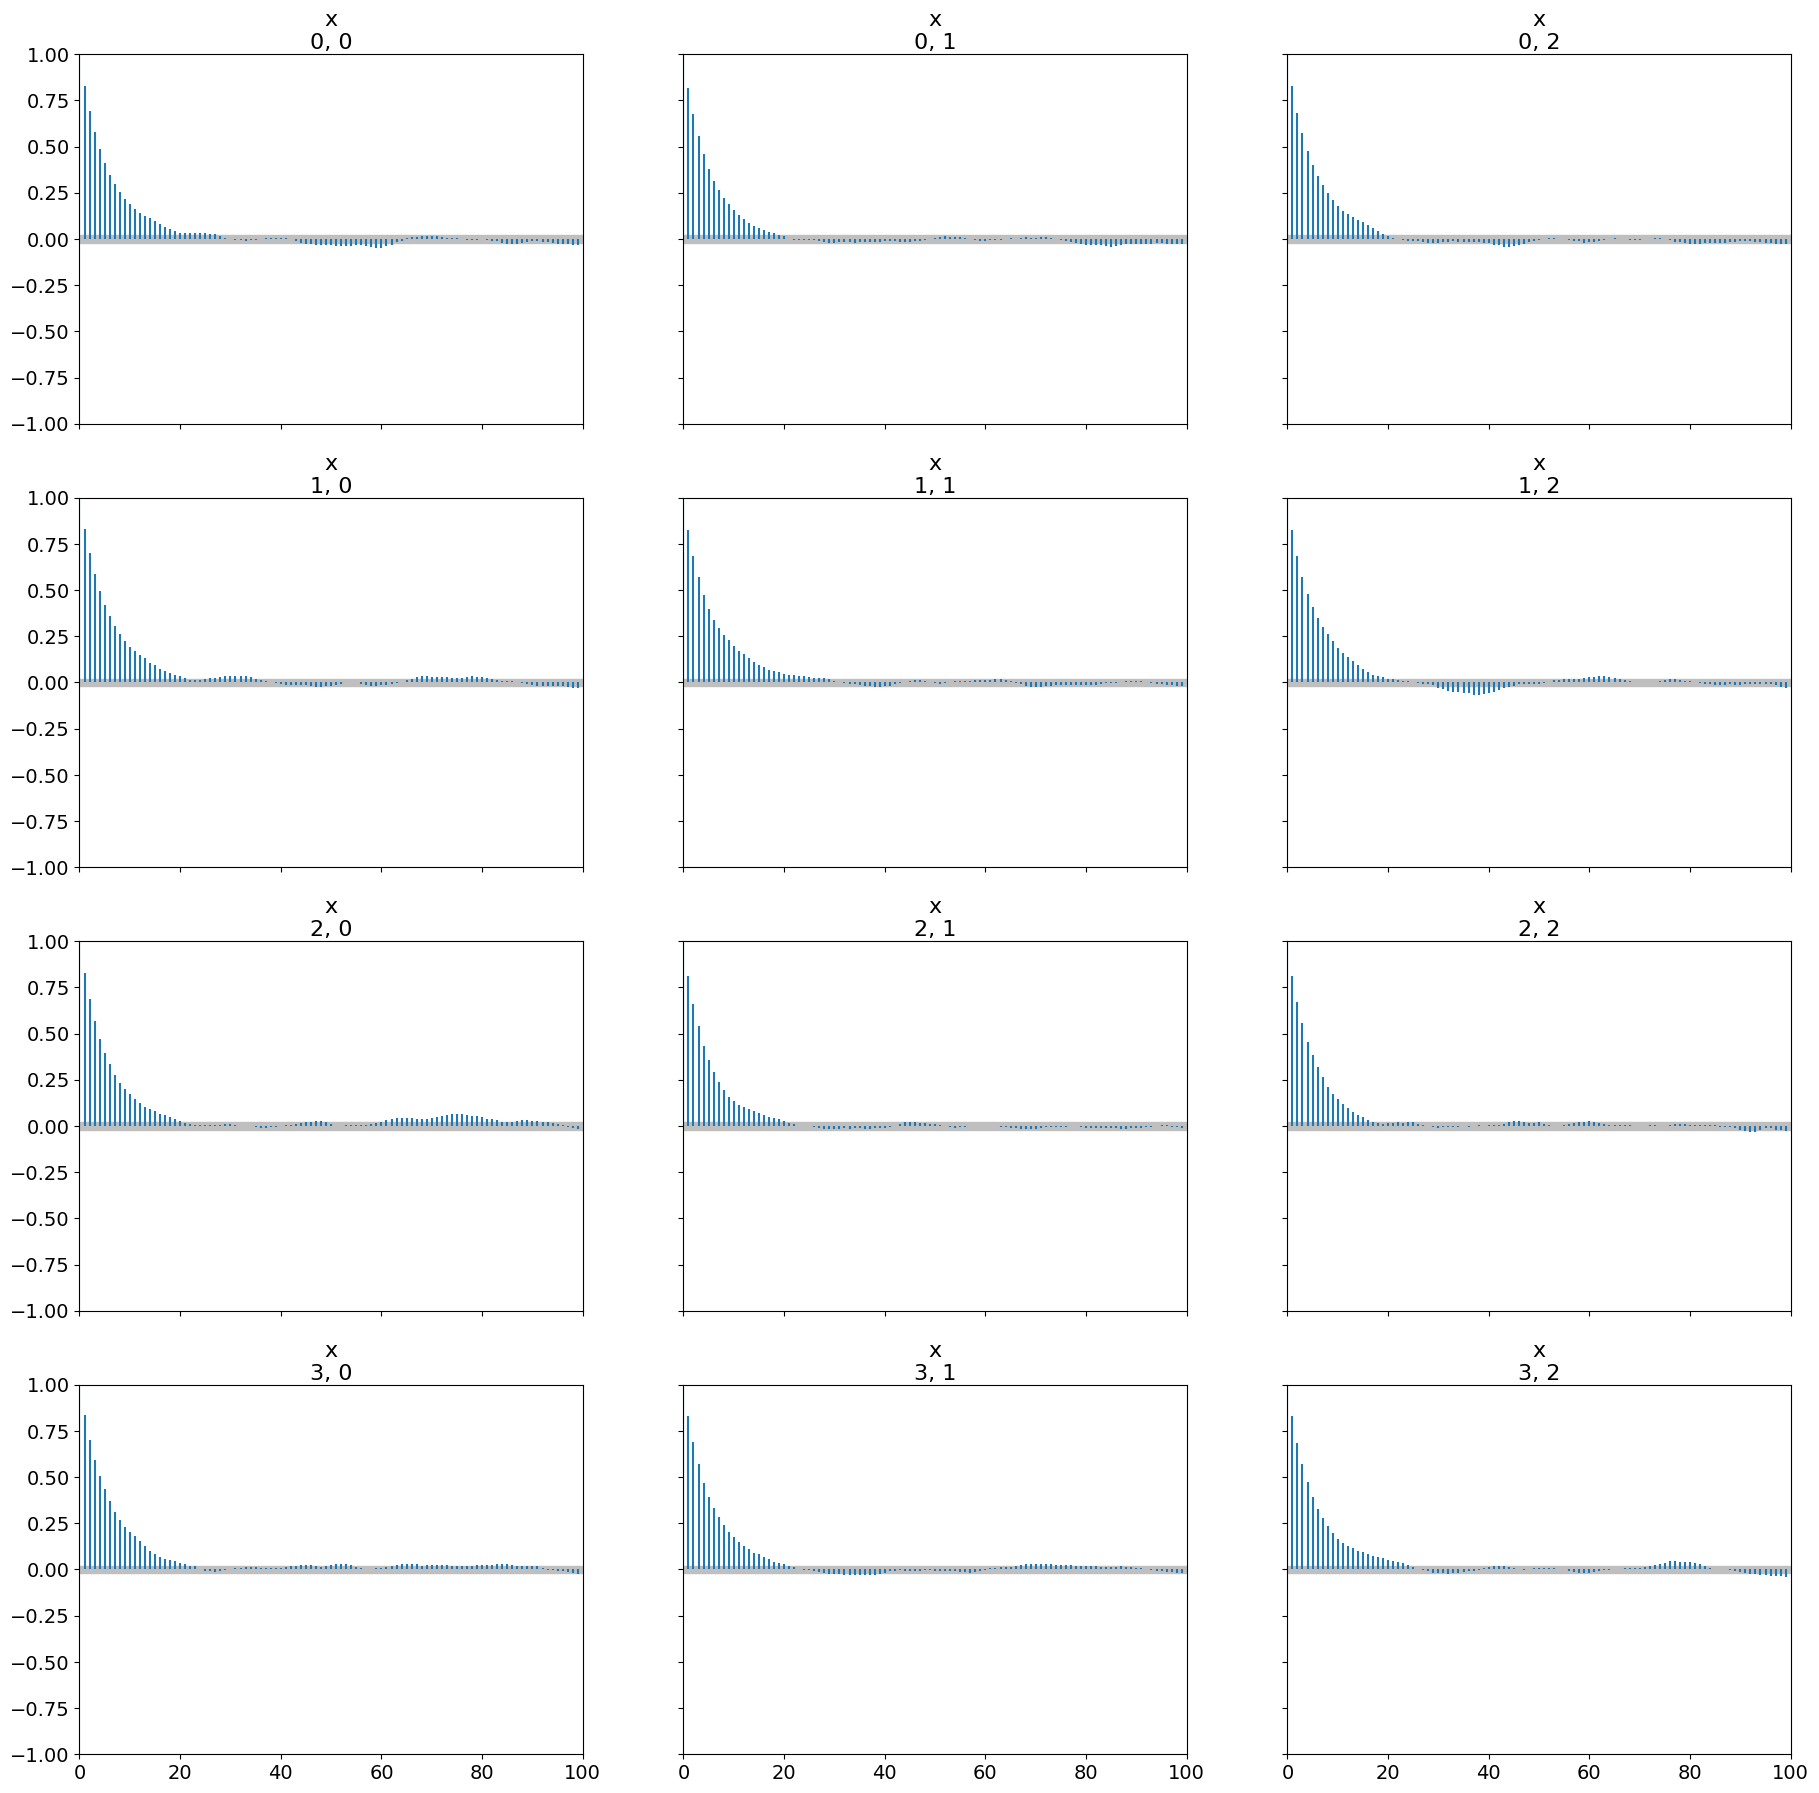
\includegraphics[width=0.5\linewidth]{Auto-Correlações.png}
    \caption{Auto-Correlações}
    \label{fig:enter-label}
\end{figure}

\begin{figure}[h]
    \centering
    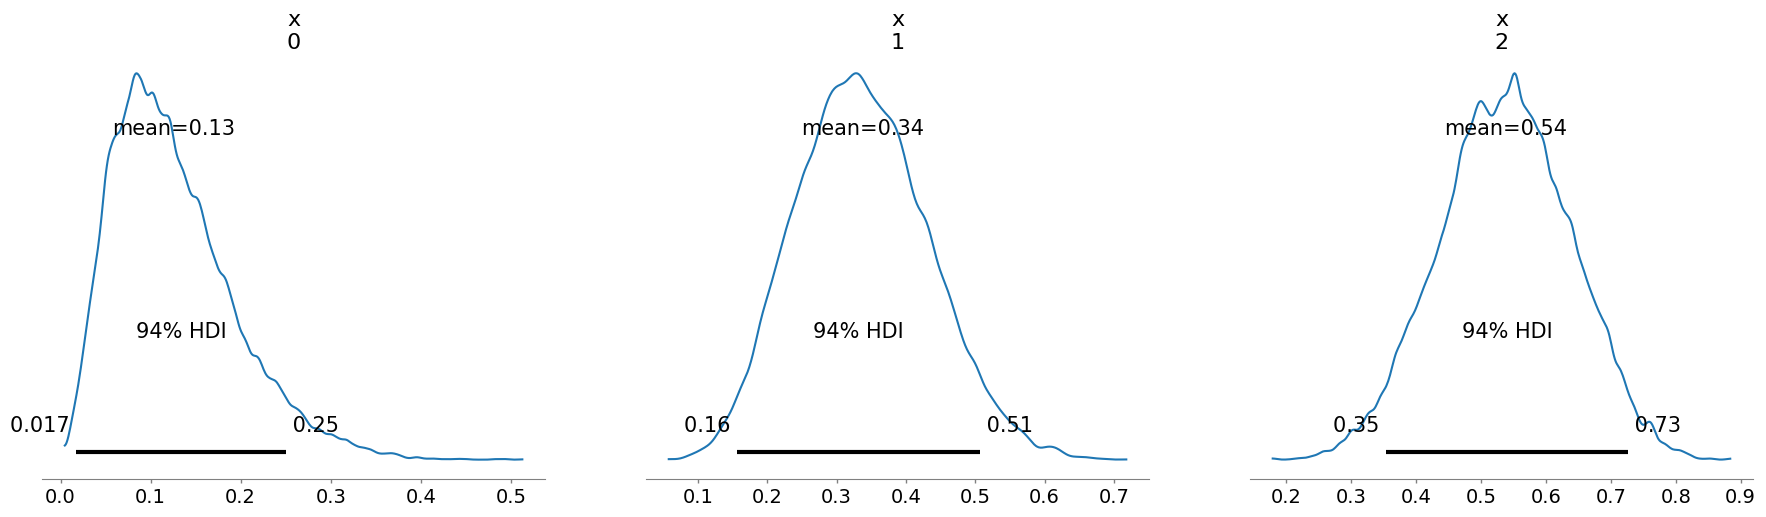
\includegraphics[width=0.5\linewidth]{Posterior Plots.png}
    \caption{Posterior Plots}
    \label{fig:enter-label}
\end{figure}

\subsection{Definição dos Cortes $v_i$}
Tendo simulados $n$ pontos por meio desse método, pode-se definir, então, os cortes $v_i$. Definie-se $v_0 = 0$ e $v_k = sup(f) = max(f(\theta))$. Assim, o supremo de $f(\theta)$ é simplesmente o maior valor de $f$ para os pontos $\theta$ gerados. Para os outros cortes, busca-se criá-los de tal forma que todos os bins tenham tamanhos semelhantes.

Para isso, defini-se o tamanho dos bins por meio da divisão inteira entre o número de pontos $n$ e o número de bins $k$. Evidentemente, quando $n \not\equiv 0 \pmod{k}$, os bins não serão todos iguais. Assim, considerando $$n = q \cdot k + r =  (k - r) \cdot q + r \cdot (q + 1)$$, em que $q$ é o quociente e $r$ o resto, existirão $r$ bins com tamanho $(q + 1)$ e $(k - r)$ com tamanho $q$.

Assim, basta obter o resultado $f(\theta)$ para cada ponto e ordenar a lista de menor para maior. Com isso, define-se os pontos de corte com base no racional descrito. Logo, tem-se que $W(v_j) - W(v_{j-1}) \approx \frac{1}{k}$.

\subsection{Encontrando $U(v)$}
Por fim, falta encontrar uma equação $U(v)$ que aproxime $W(v)$. Para isso, será utilizada uma interpolação polinomial que garanta um polinômio monótono crescente. Isso porque, sendo uma função de probabilidade acumulada, necessariamente $W(u) \leq W(v)$ se $u \leq v$.

Por isso, foi utilizado o método Piecewise Cubic Hermite Interpolating Polynomial (PCHIP) para a tarefa. A ideia básica por trás do PCHIP é interpolar localmente segmentos cúbicos de Hermite entre os pontos de dados. Aqui está uma visão geral de como funciona:

\begin{enumerate}
    \item \textbf{Calcula os gradientes locais:} Para cada par de pontos de dados adjacentes, o PCHIP calcula o gradiente (ou derivada) local. Geralmente, isso é feito usando uma diferença finita dividida que leva em conta os valores das funções nos pontos de dados vizinhos.
    
    \item \textbf{Constrói segmentos cúbicos:} Com os gradientes calculados, o PCHIP constrói segmentos cúbicos de Hermite locais entre cada par de pontos de dados. Um segmento cúbico de Hermite é uma função polinomial de terceiro grau que é especificada por seus valores e gradientes em ambos os pontos finais do segmento.
    
    \item \textbf{Suaviza a curva:} O PCHIP assegura que os segmentos cúbicos adjacentes se juntem suavemente, criando uma curva contínua e diferenciável. Isso é feito garantindo que os gradientes dos segmentos cúbicos coincidam nos pontos de dados compartilhados.
    
    \item \textbf{Interpolação:} Uma vez que os segmentos cúbicos locais foram construídos, o PCHIP pode ser usado para interpolar valores em qualquer ponto dentro do intervalo dos pontos de dados. Isso é feito aplicando o segmento cúbico apropriado para cada ponto de interpolação.
\end{enumerate}

O PCHIP é especialmente útil quando os dados têm comportamento oscilatório ou não são uniformemente espaçados. Ele tende a produzir resultados mais suaves e menos suscetíveis a oscilações indesejadas do que outros métodos de interpolação. O método PCHIP também mantém a monotonicidade ajustando os gradientes dos segmentos cúbicos de Hermite para garantir que a função interpoladora seja monótona crescente ou decrescente entre os pontos de dados.

\subsection{Erro da Função $U(v)$}
O erro da função obtida pode ser divido em dois: (i) margem de erro do estimador $\hat{p_v}$; (ii) margem de erro por discretização em bins. Para o cálculo da primeira parcela, basta entender que o estimador $\hat{p_v}$ de $p_v$ atravpes de $n$ pontos gerados aproxima de uma curva normal quando $n \rightarrow \infty$. Isto é: $$\hat{p_v} \xrightarrow{n \rightarrow \infty} N\left(W(v), \frac{W(v)(1 - W(v))}{n}\right)$$.

Dessa forma, definindo um intervalo de confiança, pode-se obter a fórmula do erro para o estimador como: $$\epsilon_n = \frac{z_{\gamma/2}}{2\sqrt{n}}$$.

Ao mesmo tempo, ao observar a discretização da função, esta gerará um erro de, no máximo, $W(v_{j + 1}) - W(v_j) \approx 1/k$. Desse modo, pode-se determinar: $$\epsilon_k = \frac{1}{k}$$.

Por fim, o erro total será: $$\epsilon = \epsilon_n + \epsilon_k$$.

Para que o erro total seja menor que $0,05\%$, é necessario que tanto $\epsilon_n$ quanto $\epsilon_k$ o sejam. O erro por discretização decresce mais rapidamente com a crescente de $k$ do que o erro do estimador com a crescente de $n$. Além disso, no processo de computação de $U(v)$, mais processos dependem do valor de $n$ do que do valor de $k$. Portanto, para preservar uma velocidade alta de computação, compensa deixar um valor mais alto de $k$ do que de $n$. Assim, valores adequados são: $$n = 1.7 \cdot 10^4$$ $$k = 5 \cdot 10^6$$

É preciso atentar-se ao fato de que, por existir um \textit{burn-in}, parte do $n$ não é de fato utilizado. No entanto, esse valor é muito pequeno em relação ao $n$, o que não gera uma necessidade de alteração brusca.

\end{document}